\chapter{Russian Post Offices in China}  
\subsection{Russian Merchant's Post}

The Russian Merchants' (or Mongolian) Post was a private
enterprise under the protection of the Russian Government initiated
in 1865, about 10 years before the official Russian Post was established
in Mongolia and China. A charge for its service was levied on incoming mail,
payable by the recipient. From January 1872 such mail received the 
standard "Doplatit" (to pay) hs.

\subsection{Earliest Known Cover}
The Russian post offices in China were a collection of post offices 
established by Imperial Russia in various cities
of China beginning in 1870.


\begin{figure}[htbp]
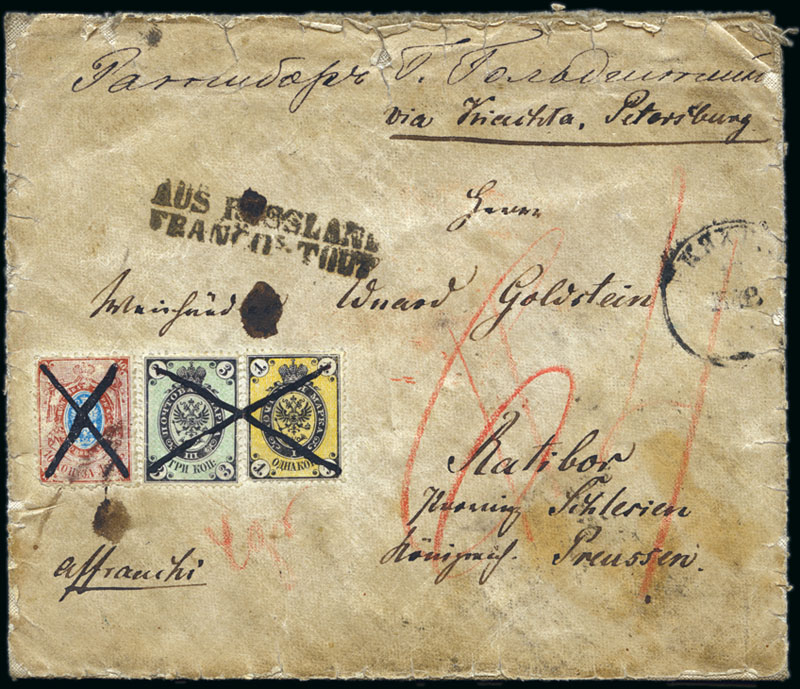
\includegraphics[width=.98\textwidth]{../russian-post-offices-in-china/10000.jpg}
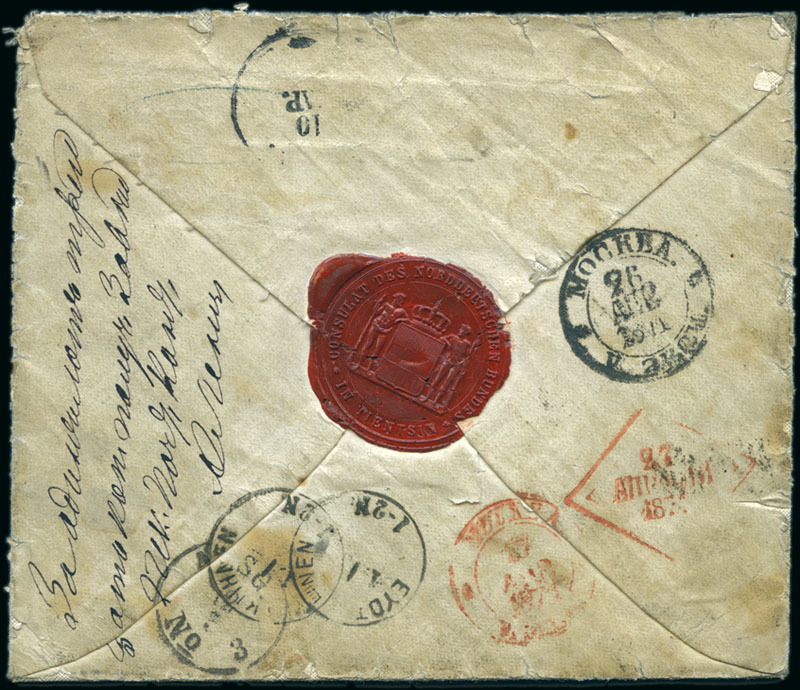
\includegraphics[width=.98\textwidth]{../russian-post-offices-in-china/10000-1.jpg}
\caption{
10000  QUASI OFFICIAL MERCHANTS POST: 1871 Envelope to Ratibor (Prussia)
from the North German Consulate in Tientsin, taken to Peking for conveyance
by Russian Merchants' Post to Russian border at Kyakhta, the fee of 30k paid
in cash with ms note on reverse, Russian 1k, 3k and 10k pen cancelled by
sender for pre-payment of UPU rate from Russia to Prussia, some peripheral
wear, still unique and the earliest known cover bearing Russian stamps in China.
Note: Described and illustrated in BJRP 94/95 (2006) p.45-46
Currently (SAN)...\euro 30,000.00
}  

\end{figure}


\begin{figure}[htbp]
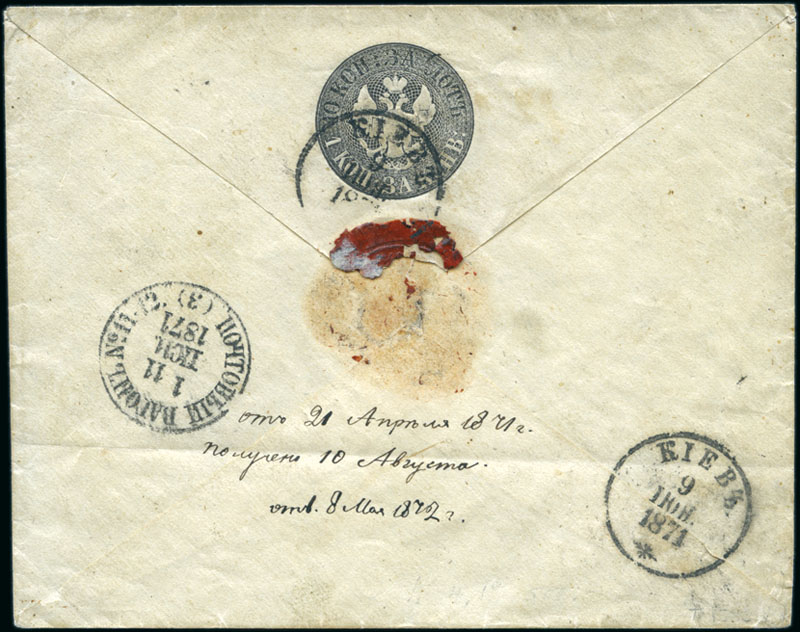
\includegraphics[width=.98\textwidth]{../russian-post-offices-in-china/10001.jpg}
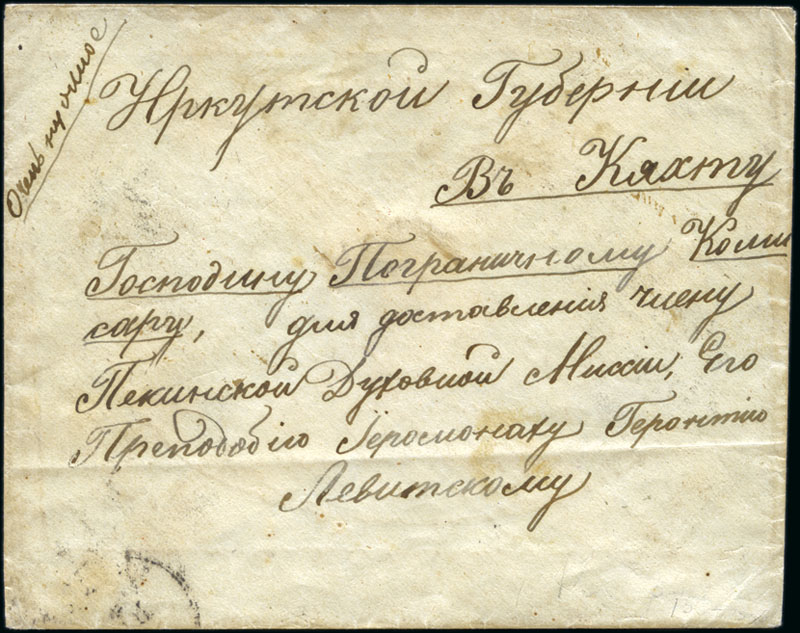
\includegraphics[width=.98\textwidth]{../russian-post-offices-in-china/10001-1.jpg}
\caption{
10001 QUASI OFFICIAL MERCHANTS POST: 1871 Incoming 10k postal 
stationery envelope (1863 issue) sent to the Border Commissar at Kyakhta 
on the Siberia / Mongolia border for transmission to a member of the 
Russian Ecclesiastical Mission at Peking, placed on Postal Wagon No.11-12 
(Kiev-Nizhnii-Novgorod), then taken by Merchants' Post across Mongolia to 
Peking, received 10.8.71 (ms note)
Currently (SAN)...\euro 1,800.00
}        
\end{figure}







